\section{Theorie}
\label{sec:Theorie}
Aufgrund der hohen Präzision werden üblicherwiese Brückenschaltungen eingesetzt. Um die Präzision zu gewährleisten wird die sogenannte Nullmethode eingesetzt.
Mit Hilfe dieser Methode werden die Schaltungen abgeglichen, damit die zu messenden Größen mit einer hohen Genauigkeit bestimmt werden können. Außerdem lässt sich jede
physikalische Größem, welche sich als elektrischer Widerstand darstellen lässt, sehr präzise messen.
\subsection{Allgmeine Brückenschaltung}
Um die Ableichbedigung zu berechnen, betrachtet man zunächst die Spannung zwischen zwei Punkten auf zwei verschieden Leitern. Die dort anliegende Potentialdifferenz U
zwischen den Punkten A und B, welche auch als Brückenspannung bezeichnet wird hängt von den Widerstandsverhältnissen ab,
weswegen man dieses Verhätnis zum Abgleichen ausnutzt.
Die allgemeine Gestalt einer Brückenschaltung wird in  Abbildung \ref{fig:allgBrücke}
\begin{figure}
    \centering
    \caption{Allgemeine Brückenschaltung} 
    \label{fig:allgBrücke}
    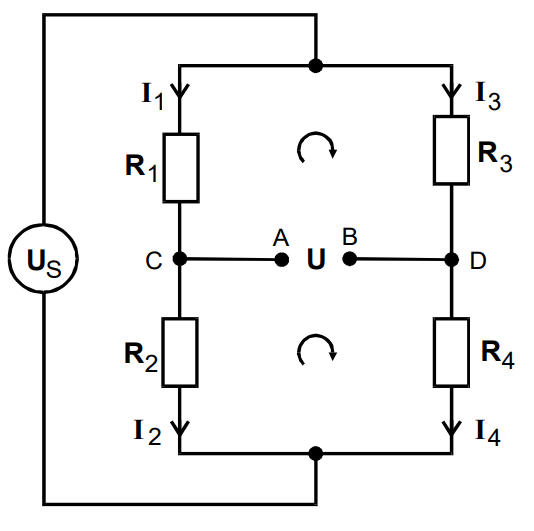
\includegraphics[width = 0.5\textwidth]{bridges/genbridge.png}
\end{figure}
dargestellt. Allgemein kann man Schaltkreise mit Hilfe der Kirchhoffschen Gesetzen beschreiben.
\subsection{Kirchoffschen Gesetze}
\subsubsection{Knotenregel}
Die erste Kirchhoffsche Regel ist die Knotenregel, welche besagt, dass die Summe aus den zufließenden und abfließenden Strömen Null ist.
Mathematisch ausgedrückt sieht die Knotenregel wie foglt aus:
\begin{equation}
    \sum_{k=1}^N I_k = 0 \label{eqn:knotrule}
\end{equation} 
\begin{figure}
    \centering
    \caption{Illustration zur Knotenregel}
    \label{fig:knotrule}
    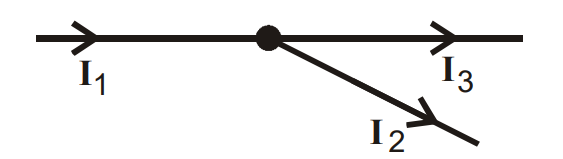
\includegraphics[width = 0.5\textwidth]{bridges/knotrule.png}
\end{figure}
Damit die Konfiguration in Abbildung \ref{fig:knotrule} gültig ist, müssen entweder die abfließenden Ströme $I_2$ und $I_3$ oder 
der zufließende Strom $I_1$ ein negatives Vorzeichen haben, so dass die Gleichung \eqref{eqn:knotrule} ihre Gültigkeit 
behält. Zwecks Konventionen besitzen die abfließenden Ströme negative Vorzeichen.
\subsubsection{Maschenregel}
Die zweite und damit letzte Kirchhoffsche Regel sagt aus, dass die Summe der Spannungen in einer sogenannten Masche ebenfalls Null ergeben muss, so dass sich die Formel
\begin{equation}
    \sum_{k=1}^N U_k = 0 \label{eqn:stitchrule}
\end{equation}
ergibt.
\begin{figure}
    \centering
    \caption{Illustration zur Maschenregel}
    \label{fig:stitchrule}
    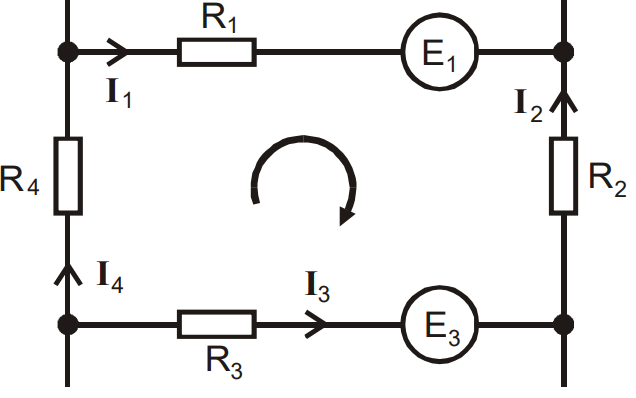
\includegraphics[width=0.5\textwidth]{bridges/stitchrule.png}
\end{figure}
Hierbei müssen manche manche Spannung über die jeweiligen Komponenten ein negatives Vorzeichen besitzen, damit die Gleichung \eqref{eqn:stitchrule} aufgeht.
Die Spannungen, wessen Pfeile des Stroms gegen den Uhrzeigersinn laufen, erhalten ein negative Vorzeichen.
\subsection{Abgleichbedingung}
Damit man die Größen der gesuchten Bauteile errechnen kann, muss die Brücke abgeglichen sein. Dies bedeutet, dass die Spannung U zwischen den Punkten A und B (s. 
Abbildung \ref{fig:allgBrücke}) gleich Null ist. Um zu messen, wie groß die Spannung U ist, benötigt man einen Nullindikator.
Nach Anwendung der beiden Kirchhoffschen Gesetzen erhält man für $U_\text{S}$ den Ausdruck  
\begin{equation}
    U = \frac{R_2 R_3 - R_1 R_4}{\left( R_3 + R_4 \right) \left( R_1 + R_2\right)} U_\text{S} \; \text{.} \label{eqn:U}
\end{equation}
Damit die Spannung U verschwindet, muss der Zähler aus Gleichung \eqref{eqn:matchingcondition} Null ergeben, so dass sich die Abgleichbedigung mathematisch zu
\begin{equation}
    R_1 R_4 = R_2 R_3 \label{fig:matchingcondition}
\end{equation}
zusammenfassen lässt. 
\subsection{Wheatstonesche Brücke}
Um einen unbekannten Ohmschen Widerstand $R_\text{x}$ auszumessen, kann die Wheatstonesche Brücke benutzt werden. 
\begin{figure}
    \centering
    \caption{Wheatstonsche Brücke}
    \label{fig:Wheatstone}
    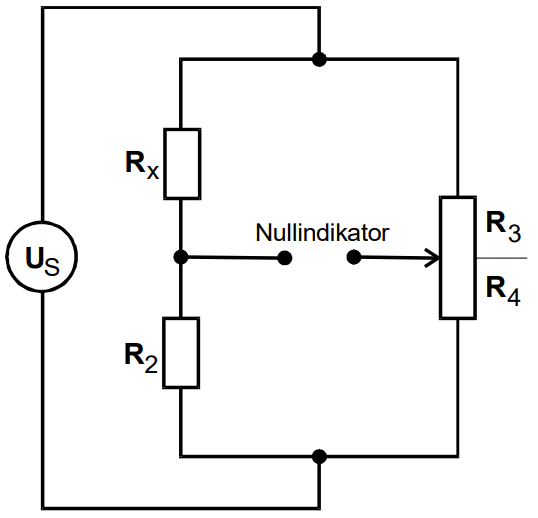
\includegraphics[width = 0.5\textwidth]{bridges/wheat.png}
\end{figure}
Die Abgleichbedigung für diese Brückenschaltung lautet
\begin{equation}
    R_\text{x} = R_2 \frac{R_3}{R_4} \; \text{.}
\end{equation}
